\chapter{Results} \label{chapter:results}

% 논문의 목적에 따라 실행한 연구 결과를 부제에 맞추어 기술하고 구체적인 데이터를 그림이나 표로 제시한다.

\section{Effect of Space Optimization}

The effect of space optimization for k-mer table and ID table is visualized in the \autoref{fig:space_opt}.
For the forementioned 900MB database in \cref{section:space-optimization}, \autoref{fig:k11_space}, when we generate \texttt{Petasearch} data structures for 11-mers, the total space usage is reduced from 17.8GB to merely 849MB (0.85GB), decreasing the space usage by $95.35\%$ compared to the original \texttt{Petasearch} data structures.
Viewing separately, the space usage of the k-mer table is reduced from 5.9GB to 405MB ($-93.34\%$), and the space usage of the ID table is reduced from 11.9GB to merely 444MB ($\-96.36\%$).
The effect of ASCII-squeezing method and simplified database index combined is exhibited in \autoref{fig:ascii-squeezing}.
The size of the sequence database was reduced by $28.27 \%$ for a 300MB-scale database.
For gigabyte-sized database, the compression efficiency is even higher -- a 82.1GB database got compressed to only 46.3GB thanks to ASCII-squeezing method and simplified index.

\section{Speed Benchmark}



\section{Sensitivity Benchmark}

\begin{figpage}
  \newgeometry{left=8mm, right=10mm}
  \captionsetup[figure]{width=.9\linewidth}
  \captionsetup[subfigure]{
    width=.9\linewidth
  }
  \centering
  \begin{figure}
    \begin{subfigure}{0.5\textwidth}
      \centering
      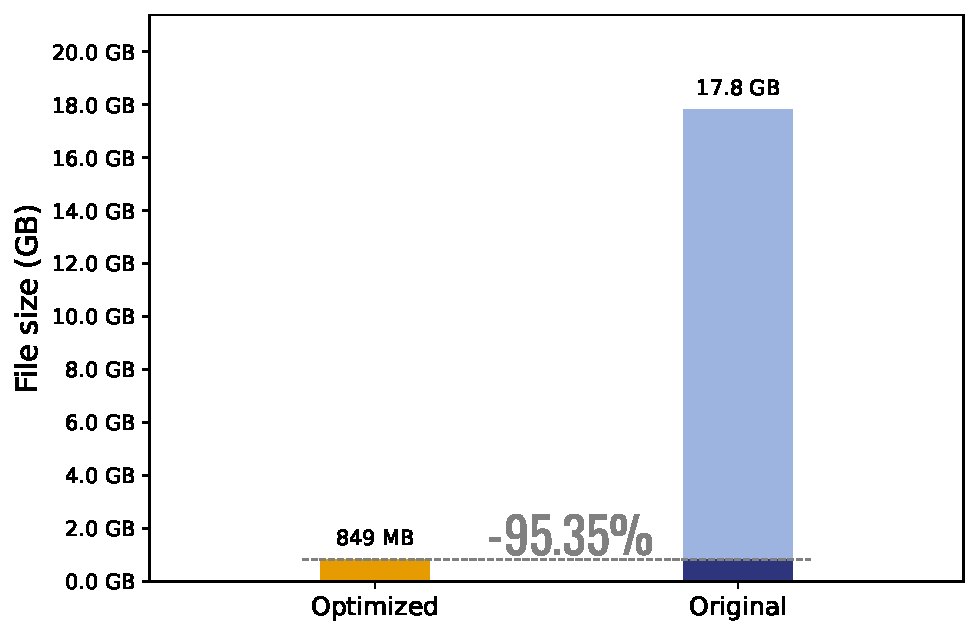
\includegraphics[width=\textwidth]{images/bitsqueeze_alternative.pdf}
      \centering
      \caption{Visualization of he total amount of reduction in space usage for the \texttt{Petasearch} data structures.
The great reduction in space usage makes the previous implausible search for 11-mer index possible.}
      \label{fig:total_effect_of_bitsqueeze}
    \end{subfigure}
    \begin{subfigure}{0.5\textwidth}
      \centering
      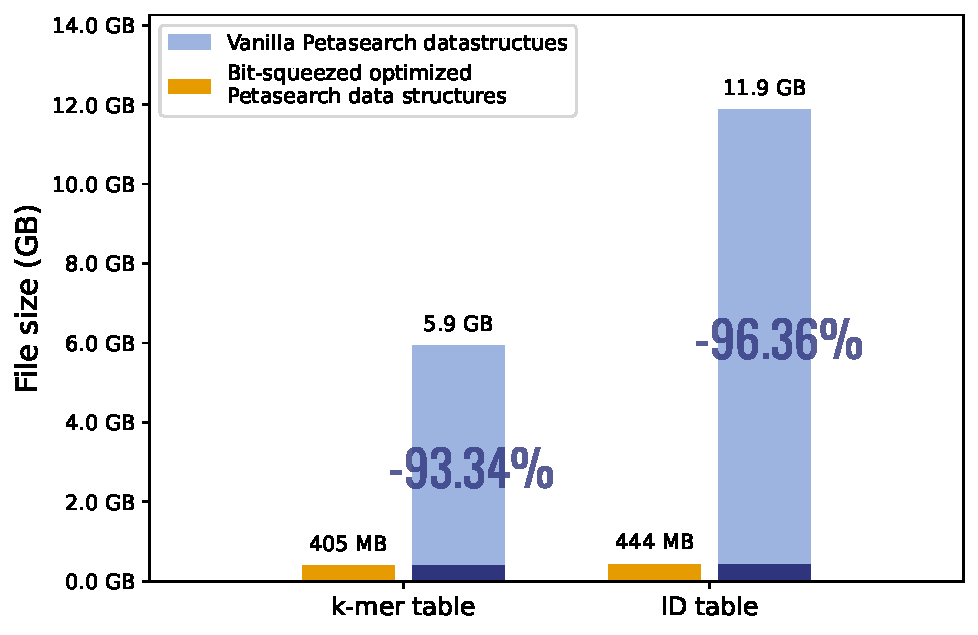
\includegraphics[width=\textwidth]{images/bitsqueeze_optimization.pdf}
      \caption{Visualization of the space reduction for k-mer table and ID table separately.
The carefully designed bit-squeezing technique and redundancy reducion for ID table are both highly effective.}
      \label{fig:separate_effect_of_bitsqueeze}
    \end{subfigure}
    \caption{\textbf{Effect of space optimization for k-mer diff-index table and ID table using bit-squeezing technique at $\mathbf{k = 11}$.} \cref{fig:total_effect_of_bitsqueeze} showed the total effect of bit-squeezing on both \texttt{Petasearch} data structures.
\cref{fig:separate_effect_of_bitsqueeze} showed the effect of bit-squeezing on the k-mer diff-index table and the ID table separately.}
    \label{fig:space_opt}
  \end{figure}
  \begin{figure}
    \begin{subfigure}{0.5\textwidth}
      \centering
      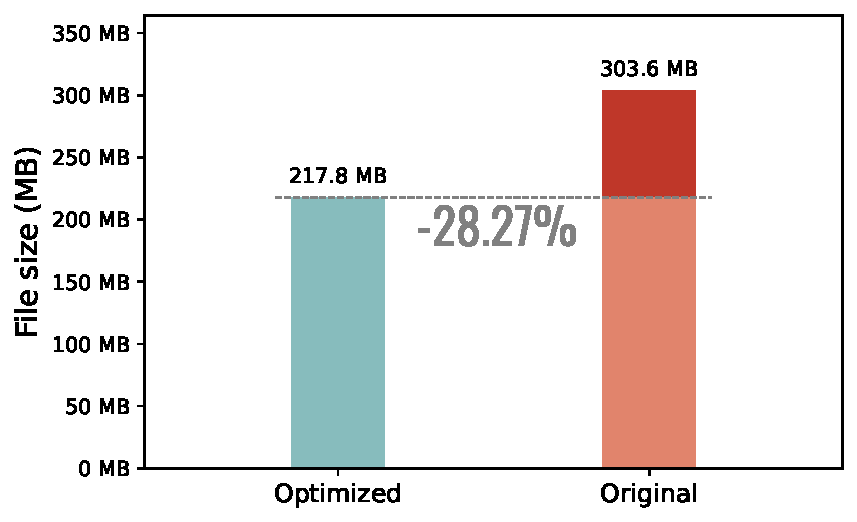
\includegraphics[width=\textwidth]{images/seqdbsize_small.pdf}
      \caption{The amount of space reduction for a 303.6 MB database. The space saving is about $28.27\%$ or one third of the size of the original database.}
      \label{fig:seqdbsize_small}
    \end{subfigure}
    \begin{subfigure}{0.5\textwidth}
      \centering
      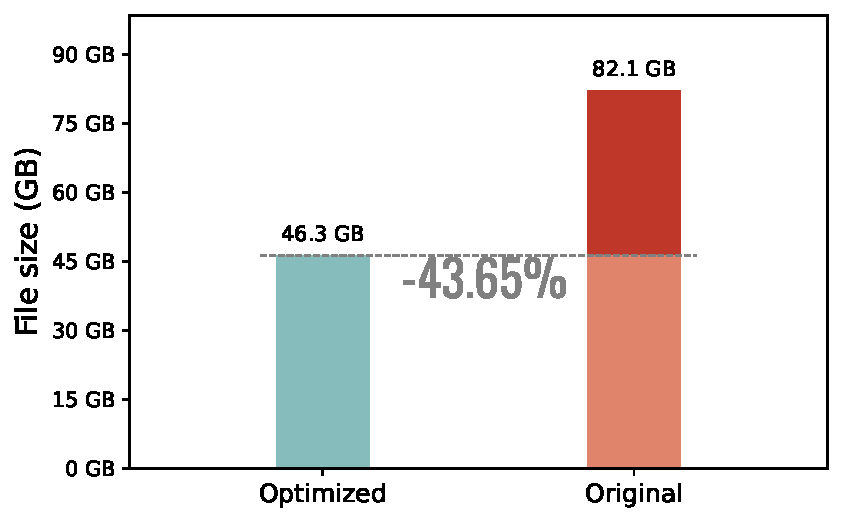
\includegraphics[width=\textwidth]{images/seqdbsize_large.pdf}
      \caption{The amount of space reduction for a 82.1 GB database. The space saving is even higher than smaller databases, reaching $43.65\%$.}
      \label{fig:seqdbsize_large}
    \end{subfigure}
    \caption{\textbf{Effect of \texttt{ASCII}-squeezing method and simplified database index.} We also briefly test the effect of the compression efficiency with respect to the size of the database.}
    \label{fig:ascii-squeezing}
  \end{figure}
  \restoregeometry
\end{figpage}
